\chapter*{{\FontH{\Huge Erdbeeren}}\\\small \color{DeepPink} Opa Werner gewidmet}
\addcontentsline{toc}{chapter}{Erdbeeren}
\lettrine[lines=3]{\color{DeepPink}S}{ommer.} Meret und Fenja besuchen ihren Opa. Die Sonne scheint und die neuen Bikinis warten darauf, endlich am Baggersee eingeweiht zu werden. Noch schnell eine Träne verstecken, während sich Mama und Papa verabschieden. Die wollen noch weiter, Freunde besuchen. Meret und Fenja verbringen zum ersten Mal alleine die Ferien beim Opa. Der wohnt jetzt noch gar nicht so lange in dem Haus, der ist erst eingezogen. Aber dass es einen See gibt und einen Fluss, wissen alle schon, da kann eigentlich nichts mehr schief gehen.

Die Schwestern wollen schon gleich in der ersten Nacht im Zelt im Garten schlafen. Die Eltern und Opa sind da zwar skeptisch, nicht dass die beiden etwa noch Angst bekommen nachts. Aber weil Meret und Fenja unglaublich oft \enquote{Bitte, bitte, bitte!} wiederholen können, setzen sie sich durch.

Opa hat einen prima Garten. Apfel- und Zwetschgenbäume stehen da, Sauerkirschen gibt es, die die beiden aber nicht so mögen, dazu Johannisbeeren, Brombeeren und natürlich die Erdbeeren. Die sind die besten, da sind sich beide einig. Frisch pflücken, klein drücken, Milch und ein bisschen Zucker dazu und dann so viel davon essen, bis man Bauchschmerzen bekommt. Traumhaft!

Und genau neben diesem Erdbeerbeet steht ihr Zelt. Knallrot ist es, was beide toll finden. Opa hat es schon aufgebaut, jetzt muss es noch eingerichtet werden. Ganz oben wird eine Taschenlampe aufgehängt und an den Seiten werden die wichtigsten Dinge verteilt. Zuerst die Plüschtiere, dann ein Kompass, falls man eine Schatzkarte findet und den Schatz suchen muss. Ganz wichtig sind auch die Buntstifte, obwohl man im Zelt eigentlich nicht so gut malen kann. Aber die sind ganz neu, die müssen unbedingt in der Nähe bleiben. Zuletzt die Urkunde aus den letzten Skiferien und natürlich ein Foto von Mama und Papa. Für den aufblasbaren Delphin ist leider kein Platz mehr, der muss draussen bleiben. Und zwischen all den Dingen ihre Schlafsäcke. Papa nennt die Schlaftüten, was beide aber kindisch finden.

Opa hat am Abend zur Begrüssung den Grill angefeuert. Es gibt Bratwürste und Kartoffelsalat. Aber wirklich etwas davon zu essen, schaffen die beiden nicht mehr. Bauchschmerzen von rosafarbener Erdbeermilch. Dann sitzen alle noch lange draussen im Garten auf weissen Plastikstühlen und erzählen, was in letzter Zeit so passiert ist. In der Schule macht es beiden Spass, aber Ferien sind schöner. Fenja nervt vor allem ein Mädchen aus ihrer Klasse, die ist einfach nur blöd. Meret ist gerade erst in die Schule gekommen, die nervt noch gar nichts. Das komme noch, meint die manchmal altkluge Fenja.

Mittlerweile haben die vielen Vögel, die ringsum auf den Dächern und Bäumen sitzen und den ganzen Tag ein lautes Konzert veranstalten, auch aufgehört zu zwitschern. Ihre Köpfe haben sie wohl schon unter die Flügel gesteckt. Ob Vögel wohl auch manchmal schnarchen? Wunderbar still ist es im Garten, nur die Grillen zirpen, die sind ja auch jetzt erst aufgestanden.  So eine Ruhe sind die beiden Städterinnen nicht gewohnt. Dort machen die ganze Nacht Autos und Strassenbahnen und sonstige Dinge Lärm. Still es es da nie. 

\afterpage{
    \begin{figure}
        \thispagestyle{empty}
        \centering
        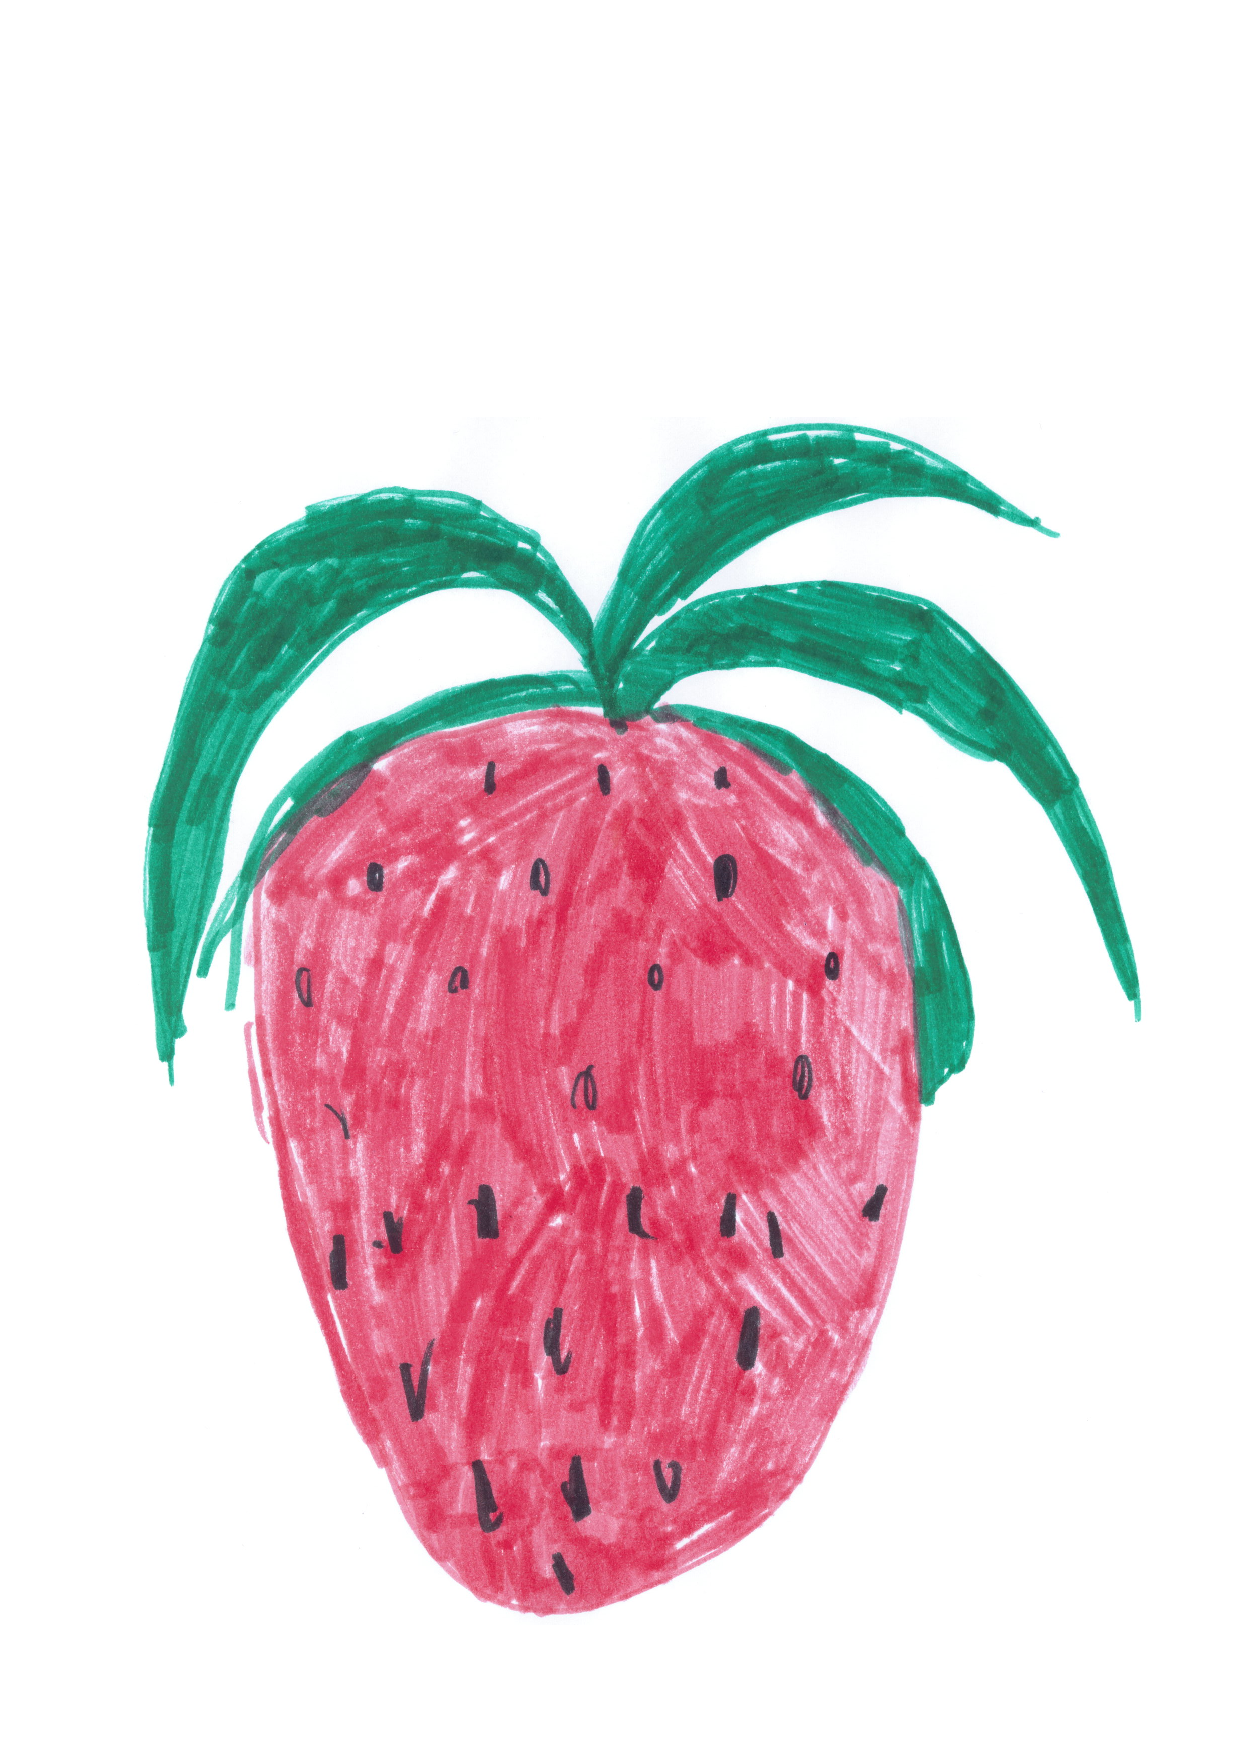
\includegraphics[width=\textwidth]{bilder/opa1.pdf}
    \end{figure}
    \clearpage
}

Als die beiden Schwestern gerade diskutieren, ob sie schon zu alt seien für Biene Maya, oder ob die neuen Folgen doch gerade noch okay sind, merken sie, dass Opa die Augen zugefallen sind. Sie müssen kichern. Sie räumen noch schnell das letzte Geschirr in die Küche, wovon Opa wieder wach wird. Aber nur so viel, dass er sich gerade noch verabschieden kann und sich schlafen legt.


Die beiden liegen noch lange wach und gucken in den klaren Sternenhimmel. Sogar Glühwürmchen gibt es hier. Meret versucht eins zu fangen, das ist gar nicht so leicht. Plötzlich sieht sie ein viel grösseres Glühwürmchen mitten im Erdbeerbeet. Aber Moment, das ist ja gar kein Glühwürmchen, das leuchtet ja rot! Die Schwestern gucken erstaunt, denn was da leuchtet, ist eine Erdbeere.

Vorsichtig pflücken sie die Erdbeere. Seltsam. Mit ihrem Taschenmesser schneiden sie die Erdbeere in der Mitte entzwei. Auch innen leuchtet sie. Sehr schwach zwar, aber es besteht kein Zweifel. Von so etwas hat noch keine der beiden gehört. Eigenartig. 

Wenn sich eine Gelegenheit ergibt, müssen die beiden Schwestern immer versuchen herauszufinden, wer von beiden in irgendetwas besser ist. Den höchsten Turm mit Lego bauen, am schnellsten die Treppe bis in den vierten Stock hochrennen oder sich trauen, eine Schnecke von Papa zu probieren, wenn der mal wieder welche isst. 

Fenja stichelt: \enquote{Wetten, dass du dich nicht traust, so eine Hälfte zu essen.}. 

Meret muss die Herausforderung annehmen, sonst hat sie das Schwesternduell verloren. Zack ist die Hälfte der Erdbeere in ihrem Mund verschwunden.

\enquote{Und jetzt du die andere Hälfte.} Fenja weigert sich erst ein bisschen. Womöglich ist die Erdbeere ja schon schlecht und damit giftig. Es kommt zur üblichen Schwesterndiskussionen, die immer nach genau demselben Muster abläuft. Es geht mit dem Vorwurf \textit{Feigling} los, wird mit \textit{selber} erwidert und dann geht das wie beim Tischtennis eine Weile so hin und her. Meret ist aber diesmal klar im Vorteil, denn sie hat die eine Hälfte ja schon gegessen. Fenja muss auch, will sie nicht den Rest der Ferien das überlegene Gesicht der kleinen Schwester sehen. Das schlimmste, was passieren kann, ist es Bauchschmerzen zu bekommen, überlegt sie. Die sind aber sicher aber spätestens morgen Abned vorbei, es gibt ja schliesslich Medikamente. Also gut, und auch die zweite Hälfte ist gegessen.

Eine Weile warten beide, ob sie Bauchschmerzen bekommen, es passiert aber nichts und beim Warten schlafen sie ein.

\begin{center}
    {\color{DeepPink}\aldineleft}
\end{center}

Der nächste Morgen beginnt zunächst ganz normal. Meret hatte doch ein bisschen Angst bekommen im Zelt, deswegen war Fenja mit ihr ins Haus gegangen, um weiter zu schlafen. Opa hatte schon vorgesorgt und ein Bett vorbereitet. Mal sehen, ob es nächste Nacht klappt. Opa geht noch schnell zum Bäcker, frische Brötchen kaufen. Die beiden Schwestern sitzen draussen auf der Veranda und trinken heissen Kakao. Die Vögel zwitschern wieder, als gäbe es einen Wettbewerb, wer das wohl am lautesten kann. Die Sonne scheint auch schon wieder mit ganzer Kraft, Fenja muss blinzeln und schliesst die Augen.

\enquote{\dots und dann sagt der freche Sperling zu mir, er hätte den Wurm zuerst gesehen. Dass muss man sich einmal vorstellen. Sperlinge sind doch weiss Gott die frechsten Vögel weit und breit.}

\enquote{Ja, ja, da sagen sie ein wahres Wort, Frau Amsel, erst neulich habe ich \dots}

Fenja erschrickt. \enquote{Hast du das auch gehört?} fragt sie Meret. Die schlürft nur weiter an ihrem Kakao und überlegt, ob man den auch mit Erdbeeren kombinieren kann.

\enquote{Was meinst Du?}

Aber auch Fenja hört es nicht mehr. Sie konzentriert sich ganz fest, aber nichts. Um noch besser zu hören, schliesst sie wieder die Augen und da sind die Stimmen wieder:

\enquote{Und überhaupt, was für ein protziges Nest sich diese Meise gebaut hat. Geschieht ihr ganz Recht, dass sie einen Kuckuck gross ziehen muss.}  

Augen wieder auf, Stimmen weg. Augen zu, Stimmen da. Auch Meret muss das ausprobieren und auch bei ihr funktioniert das. Beide sind aufgeregt. Sie verstehen die Stimmen der Vögel! Unglaublich. Sie schliessen die Augen und hören zu.

\enquote{Und haben sie gesehen meine Liebe, die Erdbeere von der alten Hexe ist auch weg!}

\enquote{Die Zauberbeere? Nein! Wer mag die wohl gegessen haben! Hoffentlich nicht die Hexe selber. Haben sie die übrigens gesehen in letzter Zeit?}

\enquote{Na ich glaube, die hat den Wald seit Wochen nicht mehr verlassen. Seit sie Herrn Rabe gefangen hat, habe ich nichts von ihr gehört. Wie es dem wohl geht? Vielleicht hat der Mann, der jetzt hier wohnt, die Erdbeere gegessen. Oder diese beiden jungen Mädchen, die zu Besuch sind. Schauen sie nur, da unten sitzen sie und lassen sich die Sonne auf den Bauch scheinen. Versteh einer die Menschen. Sitzen nur rum und suchen nie Futter. Also nein, also nein.}

Meret und Fenja sehen sich an. Die leuchtende Erdbeere wurde von einer Hexe gepflanzt? Was mag das für eine Hexe sein? Und warum hat sie das getan? Können sie jetzt für immer die Vögel verstehen? Tausend und eine Frage stellen sich die Schwestern gegenseitig, ohne sie beantworten zu können.

Als der Opa zurückkommt und schon von weitem mit der grossen Papiertüte mit all den frischen Brötchen winkt, entscheiden sich beide, dass sie das Geheimnis erst einmal für sich behalten wollen. Beim Essen fragt Fenja mit vollem Mund:

\enquote{Du, Opa, gibt es hier eine Hexe?}

Opa muss lachen.

\enquote{Ihr habt mit dem Nachbarn gesprochen, stimmt's? Die alte Frau, der vorher das Haus hier gehört hat, mag zwar ein bisschen eigentümlich sein, aber eine Hexe ist sie sicher nicht. Das behaupten die Leute nur, weil sie einen grossen Kräutergarten hat. Wenn ihr mich fragt, die Leute sind nur neidisch, weil sie die grössten Brombeeren im ganzen Ort hat. Und auf Brombeeren sind sie hier im Ort besonders stolz. Aber egal, es ist überhaupt nicht nett sie Hexe zu nennen.}

\enquote{Was ist mit der Hexe -- ähm -- alten Frau jetzt?}

\enquote{Ach, die hat noch ein kleines Hüttchen oben am Waldrand. Das Haus hier war ihr zu gross, da ist sie dahin gezogen. Aber ich weiss gar nicht, ich habe sie schon lange nicht mehr gesehen. Aber wenn ihr wollt, können wir sie besuchen, ich wollte sowieso ein bisschen mit euch wandern gehen heute, da können wir ja dort vorbei.}

Die Schwestern sind einverstanden. Sie sind zwar schon ein bisschen ängstlich, immerhin wissen sie sicher, dass es eine richtige Hexe sein muss, wenn sie so Erdbeeren pflanzen kann, aber die Neugier ist einfach grösser. Noch grösser ist allerdings die Hitze, weswegen die Wanderung auf morgen verschoben wird. Heute steht erst einmal baden an. Ab in den Fluss heisst das. Nach vielen verschmutzten Jahren, ist der jetzt wieder so sauber, dass man bedenkenlos in ihm schwimmen kann.

Auf dem Weg zum Fluss kommen die drei am Wildgehege vorbei. Es gibt Wildschweine zu sehen und auch Rehe. Sogar ein weisses Reh ist dabei. 

\enquote{Albino nennt man das}, erklärt Opa, \enquote{Aber das Reh ist sehr krank, der Tierarzt kann wohl leider nicht mehr helfen, hat mir der Förster erzählt. Aber so habt ihr es wenigstens nochmals gesehen.}

Die ganze Zeit hören sie immer wieder den Vögeln zu. Unglaublich, wie viel die zu reden haben. Wer hätte gedacht, dass das viele Gezwitscher, das man immer hört, eigentlich vor allem Tratsch und Klatsch ist? Wer wo jetzt neu ein Nest gebaut hat, wird besprochen. Bei welchem Haus jetzt eine Katze wohnt. Wie schmutzig die Tauben angeblich sind und solche Dinge eben. Am schlimmsten sind die Enten. Ständig sagen sie \enquote{Guten Tag} zueinander. So als ob sie sich das erste Mal sehen. Kaum dreht sich eine Ente um und wieder zurück, schon heisst es wieder \enquote{Guten Tag, mein Herr} oder \enquote{Guten Tag, meine Dame.} Vielmehr eigentlich nicht. Manchmal noch ein paar Floskeln zum Wetter. Überhaupt sind Vögel alle immer ausgesucht höflich. Meret und Fenja ahmen das die ganze Zeit nach, was den Opa dann doch ein wenig verwundert.

\begin{center}
    {\color{DeepPink}\aldineleft}
\end{center}

Obwohl es am nächsten Morgen schon wieder so heiss ist, wollen die beiden Schwestern unbedingt zu der alten Frau. Opa winkt ab.

\enquote{Nein meine Lieben, geht ihr gerne alleine, mir ist es zu heiss zum Wandern.} Es wird noch kurz erklärt, wo es lang geht, und dann los.

Ist das noch Aufregung oder schon Angst, was die beiden Mädchen da im Bauch zwickt? Lieber nicht zu viel darüber nachdenken, genau wie wenn man Medizin schlucken muss. 

\enquote{Und was ist, wenn sie uns wie bei Hänsel und Gretel\dots?} fängt Meret an zu fragen, wird aber von ihrer Schwester unterbrochen.

\enquote{Paperlapapp.} Sie kann zwar auch nicht sagen, auf was sie sich einlassen, aber ihr Gefühl sagt ihr, dass es schon nicht wirklich gefährlich werden kann. Sie erreichen den Wald, der hier sehr wild und dicht ist. Nach der vielen Sonne auf den Wiesen auf dem Weg, wirkt der Wald richtig düster, aber eigentlich nicht bedrohlich.

Als die Hexe dann völlig unerwartet neben ihnen steht, müssen beide vor Schreck beinahe schreien. Aber nur beinahe. 

In der Hand hält sie einen Bund aus irgendwelchen Kräutern und trägt eine schmutzige braune Kittelschürze.

\enquote{Was machen denn zwei so hübsche junge Mädchen bei dem Wetter hier im Wald. Ihr seid ja gar nicht baden?}

Keine der Schwestern weiss etwas zu sagen.

Fenja hat schon viele Geschichten über Hexen gehört oder gelesen. Eigentlich ist das sogar ihr Spezialgebiet, da kennt sie sich aus. Sie denkt sich, dass wenn das wirklich eine Hexe ist, man wohl besser nichts verheimlicht. Eine echte Hexe merkt bestimmt, wenn man schwindelt.

\enquote{Unser Opa ist der Mann, der ihr Haus gekauft hat. Er hat uns gesagt wo sie wohnen und da dachten wir, dass wir sie vielleicht einmal besuchen sollten.}

Die Alte brummt etwas vor sich hin, dann stutzt sie, überlegt und mustert die beiden von oben bis unten.

\enquote{Eine von Euch hat die Erdbeere gegessen, richtig? Und jetzt könnt ihr die Vögel verstehen. Ja, die Erdbeere hatte ich ganz vergessen, das passiert im Alter.}

\enquote{Beide.} geben die Schwestern zu, denn irgendwie haben sie nicht das Gefühl, dass die Frau böse ist. 

\enquote{Na was sagen sie denn, die Vögel? Hört es euch gut an, spätestens beim nächsten Vollmond, also heute Nacht, ist das wieder vorbei. Aber es wird auch wieder eine neue leuchtende Erdbeere wachsen, nächste Woche oder übernächste.} 

Die beiden erzählen, was sie so gehört haben, auch, dass sie, die Hexe, einen Raben gefangen haben soll. Die Hexe lacht und sagt, sie sollen mal mitkommen, sie können ja selber hören, was der Rabe zu erzählen hat. Und so gelangen sie zu dem Haus, in dem die Hexe wohnt. Ein einfaches Hüttchen, eine Art Gartenhäuschen. Hier ist es bestimmt ziemlich kalt im Winter, denkt Fenja. 

Der Rabe sitzt auf dem Rahmen einer Hollywood-Schaukel und hat einen Verband um den linken Flügel. Die Mädchen schliessen die Augen und hören den Raben sagen, dass er sich den Flügel gebrochen hat, den er aber lustigerweise Arm nennt und dass die Hexe ihm geholfen habe.

Beide sind beruhigt und kein bisschen ängstlich mehr. Es gibt kalten Kräutertee, der sehr gut schmeckt. 

\enquote{Und haben die Vögel ein weisses Reh erwähnt? Deswegen hatte ich die Erdbeeren damals überhaupt nur gepflanzt. Ich spüre, dass es diesem Reh nicht gut geht, es ist krank und es ist irgendwo eingesperrt oder gefangen. Und ich dachte, wenn ich den Vögeln zuhören kann, die aus der Luft ja alles sehen, erfahre ich vielleicht, wo das Reh ist, damit ich ihm helfen kann. Es hat Probleme mit dem Herz und ich habe die Kräuter, die ihm helfen. Leider kann man ja die Vögel nicht fragen, sondern nur hören, was sie sagen und wie ihr selber gemerkt habt, reden die Vögel meist nur Unsinniges, da habe ich das irgendwann aufgegeben.}

Die beiden Schwestern sind aufgeregt. Sie wissen natürlich, wo das weisse Reh ist. Im Wildgehege! Sie haben es ja selbst gestern erst gesehen! Die Hexe klatscht vor Freude in die Hände. 

\enquote{Wer hätte gedacht, dass ich es doch noch mit Hilfe der Erdbeeren finde!} Sie geht ins Haus und kommt mit einem Säckchen voller Kräuter zurück. 

\enquote{So ihr beiden. Seid so nett und helft mir, wir gehen gleich los.} Mit diesen Worten und einem energischen Blick, der keinen Zweifel daran lässt, dass die beiden Schwestern sie ziehen sollen, stellt sie einen alten Stuhl auf einen Bollerwagen. Kein Problem für die beiden. Es wird \textit{Das Wandern ist des Müllers Lust} und \textit{Hab mein Wagen voll geladen} gesungen und so vergeht die Zeit sehr schnell, bis sie beim Tiergehege sind.

Die Hexe streckt die Hand aus und alle Rehe kommen angelaufen. Die Schwestern sind beeindruckt. Gestern bei ihnen sind die Rehe eher weg gerannt. Auch das weisse Reh kommt.

\enquote{Da bist du ja, haben sie dich hier eingesperrt? Deswegen habe ich dich nicht gefunden.} sagt sie und hält ihm ihre Kräuter hin, die es auch frisst.

Sie begleiten die Hexe wieder nach Hause und versprechen, sie nochmals besuchen zu kommen, so lange sie noch beim Opa sind. Beide Schwestern sind erleichtert, dass die Vögel auch mit geschlossenen Augen wieder zwitschern. Der Zauber der leuchtenden Erdbeere ist wieder verschwunden.

Am Abend gibt es schon wieder Bratwürste und rosa Erdbeermilch. Während Opa die Bratwürste dreht, sind die Vögel nochmals besonders laut.

\enquote{Was die wohl zu erzählen haben?} meint er. \enquote{Bestimmt erzählen die sich die verrücktesten Geschichten.}

Meret und Fenja müssen lachen und sagen wie aus einem Mund:

\enquote{Na da wäre ich mir nicht so sicher, Opa.} \hfill {\color{DeepPink}\decofourleft}

